%========================================
% LESSON CONTENT: Expresiones Racionales
%========================================

\lesson{Expresiones Racionales}

\subsectiontitle{Definiciones}

\begin{definition}
\textbf{Expresión Fraccionaria}: Es el cociente de dos expresiones algebraicas cualesquiera.

\vspace{0.5em}

\textbf{Expresión racional}: Es una expresión fraccionaria donde el numerador y el denominador son polinomios.
\end{definition}

Por ejemplo:
$$\frac{2x}{x-1} \qquad \frac{x}{x^2+1} \qquad \frac{x^3-x}{x^2-5x+6}$$

%========================================
\subsectiontitle{Dominio de una expresión algebraica}

\begin{definition}
El dominio de una expresión algebraica es el conjunto de números reales que se permite tenga la variable.
\end{definition}

Antes de trabajar con expresiones racionales, es fundamental identificar los valores que hacen que la expresión esté definida. Esto nos ayudará a evitar errores al simplificar y operar con estas expresiones.

\begin{example}
\textbf{Ejemplo 1:} Encuentre los dominios de las siguientes expresiones.

\begin{enumerate}
    \item $2x^2 + 3x - 1$
    \item $\dfrac{x}{x^2-5x+6}$
    \item $\dfrac{\sqrt{x}}{x-5}$
\end{enumerate}

\solution

\begin{enumerate}
    \item El polinomio está definido para toda $x$. Entonces, el dominio es el conjunto números reales $\mathbb{R}$.

    \item La expresión no puede tomar aquellos valores que hagan 0 el denominador. Por lo tanto se factoriza el denominador para ver claramente esos valores que no puede tomar.

    $$\frac{x}{x^2-5x+6} = \frac{x}{(x-2)(x-3)}$$

    Los valores $x = 2$ o $x = 3$ serían los valores para los cuales la expresión no está definida. Por lo tanto, el dominio es $\{x|x \neq 2 \text{ y } x \neq 3\}$

    \item El numerador solo está definido para valores $x \geq 0$. Mientras que el denominador para valores $x \neq 5$. Por lo tanto, el dominio es $\{x|x \geq 0 \text{ y } x \neq 5\}$
\end{enumerate}
\end{example}

\begin{example}
\textbf{Ejemplo 2:} Encuentre el dominio de $\dfrac{x+1}{x^2+x-12}$

\solution

Factorizamos el denominador:
$$x^2+x-12 = (x+4)(x-3)$$

Por lo tanto:
$$\frac{x+1}{x^2+x-12} = \frac{x+1}{(x+4)(x-3)}$$

El dominio es $\{x|x \neq -4 \text{ y } x \neq 3\}$
\end{example}

\begin{warning}
\textbf{Errores Comunes:}

\begin{itemize}
    \item[$\times$] \textbf{Error}: Olvidar factorizar el denominador completamente y perderse algunos valores excluidos.

    \item[$\times$] \textbf{Error}: Confundir el numerador con el denominador al determinar restricciones. Solo el denominador no puede ser cero.

    \item[$\checkmark$] \textbf{Correcto}: Siempre factorizar completamente el denominador e identificar todos los valores que lo hacen cero.
\end{itemize}
\end{warning}

%========================================
\subsectiontitle{Simplificación de expresiones racionales}

Una vez determinado el dominio, podemos simplificar expresiones racionales. La clave está en factorizar completamente antes de cancelar.

\begin{theorem}
Factorizar el numerador y el denominador y cancele los factores comunes al numerador y denominador, usando la propiedad:
$$\frac{AC}{BC} = \frac{A}{B}$$
\end{theorem}

\vspace{-0.3cm}
\begin{example}
\textbf{Ejemplo 1:} Simplifique $\dfrac{x^2-1}{x^2-2x-3}$

\solution

$$\frac{x^2-1}{x^2-2x-3} = \frac{(x+1)(x-1)}{(x+1)(x-3)} = \frac{\cancel{(x+1)}(x-1)}{\cancel{(x+1)}(x-3)} = \frac{x-1}{x-3}$$

\end{example}

\vspace{-0.3cm}
\begin{example}
\textbf{Ejemplo 2:} Simplifique $\dfrac{x^2-4x-12}{x^2-36}$

\solution

Factorizamos numerador y denominador. Luego cancelamos el factor común:
$$\frac{x^2-4x-12}{x^2-36} = \frac{\cancel{(x-6)}(x+2)}{\cancel{(x-6)}(x+6)} = \frac{x+2}{x+6}$$

\textbf{Nota}: El dominio original excluye $x = 6$ y $x = -6$, aunque la forma simplificada solo muestra $x \neq -6$.
\end{example}

\vspace{-0.3cm}
\begin{warning}
\textbf{Errores Comunes:}

\begin{itemize}
    \item[$\times$] \textbf{Error}: Cancelar términos en lugar de factores. Por ejemplo: $\dfrac{x+3}{x+5} \neq \dfrac{3}{5}$

    \item[$\times$] \textbf{Error}: No factorizar completamente antes de cancelar.

    \item[$\times$] \textbf{Error}: Olvidar que el dominio original se mantiene después de simplificar.

    \item[$\checkmark$] \textbf{Correcto}: Solo se pueden cancelar factores comunes, no términos individuales.
\end{itemize}
\end{warning}

\newpage

%========================================
\subsectiontitle{Multiplicación de expresiones racionales}

Ahora que podemos simplificar expresiones individuales, extendemos estas técnicas a productos de expresiones racionales.

\begin{theorem}
Para multiplicar dos fracciones se multiplica sus numeradores y sus denominadores respectivamente, usando la propiedad:
$$\frac{A}{B} \cdot \frac{C}{D} = \frac{AC}{BD}$$

\vspace{0.5em}
\textbf{Estrategia}: Es más eficiente factorizar primero y cancelar factores comunes antes de multiplicar.
\end{theorem}

\begin{example}
\textbf{Ejemplo 1:} Multiplique $\dfrac{x^2+2x-3}{x^2+8x+16} \cdot \dfrac{3x+12}{x-1}$

\solution

$$\frac{x^2+2x-3}{x^2+8x+16} \cdot \frac{3x+12}{x-1} = \frac{(x-1)(x+3)}{(x+4)^2} \cdot \frac{3(x+4)}{x-1}$$

$$= \frac{3\cancel{(x-1)}(x+3)\cancel{(x+4)}}{\cancel{(x-1)}(x+4)^{\cancel{2}}} = \frac{3(x+3)}{x+4}$$

% TikZ diagram for multiplication process
\begin{center}
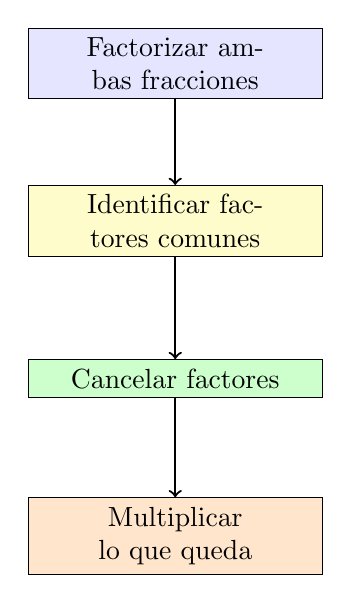
\begin{tikzpicture}[node distance=2cm, scale=0.9]
    \node (step1) [draw, rectangle, fill=blue!10, text width=3.5cm, align=center] {Factorizar ambas fracciones};
    \node (step2) [draw, rectangle, fill=yellow!20, text width=3.5cm, align=center, below of=step1] {Identificar factores comunes};
    \node (step3) [draw, rectangle, fill=green!20, text width=3.5cm, align=center, below of=step2] {Cancelar factores};
    \node (step4) [draw, rectangle, fill=orange!20, text width=3.5cm, align=center, below of=step3] {Multiplicar lo que queda};

    \draw[->, thick] (step1) -- (step2);
    \draw[->, thick] (step2) -- (step3);
    \draw[->, thick] (step3) -- (step4);
\end{tikzpicture}
\end{center}
\end{example}

\begin{example}
\textbf{Ejemplo 2:} Multiplique $\dfrac{x^2-9}{x^2+x-2} \cdot \dfrac{x+2}{x+3}$

\solution

Factorizamos:
$$\frac{(x-3)(x+3)}{(x+2)(x-1)} \cdot \frac{x+2}{x+3}$$

Cancelamos factores comunes:
$$= \frac{(x-3)\cancel{(x+3)}}{\cancel{(x+2)}(x-1)} \cdot \frac{\cancel{x+2}}{\cancel{x+3}} = \frac{x-3}{x-1}$$
\end{example}

\begin{warning}
\textbf{Errores Comunes:}

\begin{itemize}
    \item[$\times$] \textbf{Error}: Multiplicar antes de factorizar y simplificar, lo que hace el trabajo más complicado.

    \item[$\times$] \textbf{Error}: Cancelar incorrectamente a través de signos de suma o resta.

    \item[$\checkmark$] \textbf{Correcto}: Factorizar todo primero, luego cancelar, y finalmente multiplicar si es necesario.
\end{itemize}
\end{warning}

%========================================
\subsectiontitle{División de expresiones racionales}

La división se convierte fácilmente en multiplicación, lo que nos permite usar las mismas técnicas de factorización y simplificación.

\begin{theorem}
Para dividir expresiones racionales, transformar la división en una multiplicación, usando la propiedad:
$$\frac{A}{B} \div \frac{C}{D} = \frac{A}{B} \cdot \frac{D}{C}$$

\vspace{0.5em}
\textbf{Regla clave}: ``Multiplicar por el recíproco del divisor''
\end{theorem}

\newpage

\begin{example}
\textbf{Ejemplo 1:} Divida $\dfrac{x^2-4}{x+1} \div \dfrac{x+2}{x^2-1}$

\solution

Convertimos a multiplicación:
$$\frac{x^2-4}{x+1} \cdot \frac{x^2-1}{x+2}$$

Factorizamos:
$$= \frac{(x-2)(x+2)}{x+1} \cdot \frac{(x-1)(x+1)}{x+2}$$

Cancelamos:
$$= \frac{(x-2)\cancel{(x+2)}}{\cancel{x+1}} \cdot \frac{(x-1)\cancel{(x+1)}}{\cancel{x+2}} = (x-2)(x-1) = x^2-3x+2$$
\end{example}

\begin{example}
\textbf{Ejemplo 2:} Divida $\dfrac{x^2+5x+6}{x^2-4} \div \dfrac{x+3}{x-2}$

\solution

$$\frac{x^2+5x+6}{x^2-4} \cdot \frac{x-2}{x+3}$$

$$= \frac{(x+2)(x+3)}{(x-2)(x+2)} \cdot \frac{x-2}{x+3}$$

$$= \frac{\cancel{(x+2)}\cancel{(x+3)}}{\cancel{(x-2)}\cancel{(x+2)}} \cdot \frac{\cancel{x-2}}{\cancel{x+3}} = 1$$
\end{example}

\begin{warning}
\textbf{Errores Comunes:}

\begin{itemize}
    \item[$\times$] \textbf{Error}: Invertir la fracción incorrecta. Debe invertirse la segunda fracción (el divisor).

    \item[$\times$] \textbf{Error}: Intentar ``cancelar'' antes de convertir la división en multiplicación.

    \item[$\checkmark$] \textbf{Correcto}: Primero convertir a multiplicación, luego factorizar y simplificar.
\end{itemize}
\end{warning}

%========================================
\subsectiontitle{Suma y resta de expresiones racionales}

Para combinar expresiones racionales mediante suma o resta, necesitamos un denominador común, similar al proceso con fracciones numéricas.

\begin{theorem}
Si las fracciones tienen el mismo denominador, entonces se puede usar la propiedad:
$$\frac{A}{C} + \frac{B}{C} = \frac{A+B}{C}$$

Si las fracciones no tienen el mismo denominador, entonces obtener el mínimo común denominador (MCD) como sigue:
\begin{itemize}
    \item Factorizar cada denominador.
    \item Tomar el producto de los factores distintos. Usar la potencia mayor de cada factor correspondiente.
\end{itemize}
\end{theorem}

% TikZ diagram: Finding LCD
\begin{center}
\begin{tikzpicture}[node distance=1.5cm]
    \node (den1) [draw, ellipse, fill=blue!20] {Denominador 1};
    \node (den2) [draw, ellipse, fill=red!20, right=2cm of den1] {Denominador 2};
    \node (factor) [draw, rectangle, fill=yellow!20, below=1cm of den1, xshift=3cm] {Factorizar ambos};
    \node (lcd) [draw, rectangle, fill=green!20, below=1cm of factor, text width=6cm, align=center] {MCD = Producto de factores distintos (potencia mayor)};

    \draw[->, thick] (den1) -- (factor);
    \draw[->, thick] (den2) -- (factor);
    \draw[->, thick] (factor) -- (lcd);
\end{tikzpicture}
\end{center}

\begin{example}
\textbf{Ejemplo 1: Mismo denominador}

Efectúe $\dfrac{3x+2}{x-5} + \dfrac{x-7}{x-5}$

\solution

Como tienen el mismo denominador, sumamos los numeradores:
$$\frac{3x+2}{x-5} + \frac{x-7}{x-5} = \frac{(3x+2)+(x-7)}{x-5} = \frac{4x-5}{x-5}$$
\end{example}

\begin{example}
\textbf{Ejemplo 2: Diferente denominador}

Efectúe $\dfrac{5}{x+1} + \dfrac{2x}{x-2}$

\solution

$MCD = (x+1)(x-2)$

\begin{align*}
\frac{5}{x+1} + \frac{2x}{x-2} &= \frac{5(x-2)}{(x+1)(x-2)} + \frac{2x(x+1)}{(x+1)(x-2)}\\
&= \frac{5(x-2) + 2x(x+1)}{(x+1)(x-2)}\\
&= \frac{5x-10+2x^2+2x}{(x+1)(x-2)}\\
&= \frac{2x^2+7x-10}{(x+1)(x-2)}
\end{align*}
\end{example}

\vspace{-0.4cm}
\begin{example}
\textbf{Ejemplo 3: Con potencias}

Efectúe $\dfrac{2}{x^2-1} - \dfrac{3}{(x+1)^2}$

\solution

Factorizamos: $x^2-1 = (x-1)(x+1)$

$MCD = (x+1)^2(x-1)$

\vspace{-0.5cm}
\begin{align*}
\frac{2}{(x-1)(x+1)} - \frac{3}{(x+1)^2} &= \frac{2(x+1)}{(x+1)^2(x-1)} - \frac{3(x-1)}{(x+1)^2(x-1)}\\
&= \frac{2(x+1) - 3(x-1)}{(x+1)^2(x-1)}\\
&= \frac{2x+2-3x+3}{(x+1)^2(x-1)}\\
&= \frac{-x+5}{(x+1)^2(x-1)} = \frac{5-x}{(x+1)^2(x-1)}
\end{align*}
\end{example}

\vspace{-0.4cm}
\begin{warning}
\textbf{Errores Comunes:}

\begin{itemize}
    \item[$\times$] \textbf{Error}: Olvidar usar paréntesis al restar. $\dfrac{A}{C} - \dfrac{B}{C} = \dfrac{A-B}{C}$, sin paréntesis en $B$.

    \item[$\times$] \textbf{Error}: No encontrar correctamente el MCD, especialmente cuando hay potencias de factores.

    \item[$\times$] \textbf{Error}: Errores de signo al distribuir términos negativos.

    \item[$\checkmark$] \textbf{Correcto}: Usar paréntesis, encontrar el MCD correcto, y distribuir cuidadosamente.
\end{itemize}
\end{warning}

%========================================
\subsectiontitle{Fracciones compuestas}

Las fracciones compuestas aparecen frecuentemente en cálculo y otras áreas avanzadas. Simplificarlas requiere combinar todas las técnicas anteriores.

\begin{definition}
Una fracción compuesta es aquella cuyo numerador, denominador, o ambos, son expresiones fraccionarias.
\end{definition}

\begin{theorem}
Se operan como sigue:
\begin{itemize}
    \item Se convierte el numerador a una sola fracción, si fuese necesario también el denominador.
    \item El resultado anterior se reescribe como un producto de fracciones y se efectúa, usando la siguiente propiedad:
\end{itemize}
$$\frac{\dfrac{A}{B}}{\dfrac{C}{D}} = \frac{A}{B} \div \frac{C}{D} = \frac{A}{B} \cdot \frac{D}{C} = \frac{AD}{BC}$$
\end{theorem}

% TikZ diagram: Complex fraction simplification
\begin{center}
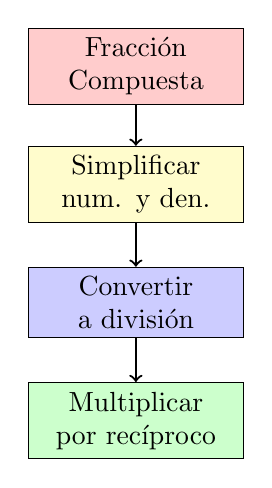
\begin{tikzpicture}[node distance=1.5cm]
    \node (complex) [draw, rectangle, fill=red!20, text width=2.5cm, align=center] {Fracción Compuesta};
    \node (simple) [draw, rectangle, fill=yellow!20, text width=2.5cm, align=center, below of=complex] {Simplificar num. y den.};
    \node (division) [draw, rectangle, fill=blue!20, text width=2.5cm, align=center, below of=simple] {Convertir a división};
    \node (multiply) [draw, rectangle, fill=green!20, text width=2.5cm, align=center, below of=division] {Multiplicar por recíproco};

    \draw[->, thick] (complex) -- (simple);
    \draw[->, thick] (simple) -- (division);
    \draw[->, thick] (division) -- (multiply);
\end{tikzpicture}
\end{center}

\newpage
\begin{example}
\textbf{Ejemplo 1:} Simplifique $\dfrac{\dfrac{x}{y}-1}{1+\dfrac{y}{x}}$

\solution

\begin{align*}
\frac{\dfrac{x}{y}-1}{1+\dfrac{y}{x}} &= \frac{\dfrac{x}{y}-\dfrac{y}{y}}{\dfrac{x}{x}+\dfrac{y}{x}}\\
&= \frac{\dfrac{x-y}{y}}{\dfrac{x+y}{x}}\\
&= \frac{x-y}{y} \div \frac{x+y}{x}\\
&= \frac{x-y}{y} \cdot \frac{x}{x+y}\\
&= \frac{x(x-y)}{y(x+y)}
\end{align*}
\end{example}

\begin{example}
\textbf{Ejemplo 2:} Simplifique $\dfrac{1-\dfrac{1}{x^2}}{\dfrac{1}{x}-\dfrac{1}{x^2}}$

\solution

Convertimos el numerador y denominador a fracciones únicas:
$$\frac{\dfrac{x^2-1}{x^2}}{\dfrac{x-1}{x^2}}$$

Dividimos:
\begin{align*}
&= \frac{x^2-1}{x^2} \cdot \frac{x^2}{x-1}\\
&= \frac{x^2-1}{x-1}
\end{align*}

Factorizamos:
$$= \frac{(x-1)(x+1)}{x-1} = x+1$$
\end{example}

\begin{warning}
\textbf{Errores Comunes:}

\begin{itemize}
    \item[$\times$] \textbf{Error}: Intentar simplificar sin convertir primero el numerador y denominador a fracciones únicas.

    \item[$\times$] \textbf{Error}: Confundir qué fracción se invierte en la división.

    \item[$\checkmark$] \textbf{Correcto}: Simplificar el numerador y denominador por separado primero, luego dividir.
\end{itemize}
\end{warning}
